\documentclass[portrait,final,a0paper]{baposter}


\tracingstats=2
\usepackage{url}
\usepackage{calc}
\usepackage{graphicx}
\usepackage{amsmath}
\usepackage{amssymb}
\usepackage{relsize}
\usepackage{multirow}
\usepackage{moresize}
\usepackage{biblatex}
\renewcommand*{\bibfont}{\scriptsize}
\addbibresource{References.bib}
\usepackage{graphicx}
\usepackage{multicol}

\usepackage{pgfbaselayers}
\pgfdeclarelayer{background}
\pgfdeclarelayer{foreground}
\pgfsetlayers{background,main,foreground}

\usepackage{times}
\usepackage{helvet}
%\usepackage{bookman}
\usepackage{palatino}

\newcommand{\captionfont}{\footnotesize}

\selectcolormodel{cmyk}

%\graphicspath{{images/}}

%%%%%%%%%%%%%%%%%%%%%%%%%%%%%%%%%%%%%%%%%%%%%%%%%%%%%%%%%%%%%%%%%%%%%%%%%%%%%%%%
%%%% Some math symbols used in the text
%%%%%%%%%%%%%%%%%%%%%%%%%%%%%%%%%%%%%%%%%%%%%%%%%%%%%%%%%%%%%%%%%%%%%%%%%%%%%%%%
% Format 

\renewcommand{\Pr}{\mbox{P}}
\newcommand{\e}{\mbox{e}}
%%%%%%%%%%%%%%%%%%%%%%%%%%%%%%%%%%%%%%%%%%%%%%%%%%%%%%%%%%%%%%%%%%%%%%%%%%%%%%%%
% Multicol Settings
%%%%%%%%%%%%%%%%%%%%%%%%%%%%%%%%%%%%%%%%%%%%%%%%%%%%%%%%%%%%%%%%%%%%%%%%%%%%%%%%
\setlength{\columnsep}{0.7em}
\setlength{\columnseprule}{0mm}

\newcommand{\compresslist}{%
\setlength{\itemsep}{1pt}%
\setlength{\parskip}{0pt}%
\setlength{\parsep}{0pt}%
}

\begin{document}

% Define some colors
\definecolor{silver}{cmyk}{0,0,0,0.3}
\definecolor{black}{cmyk}{0,0,0.0,1.0}


\definecolor{imperialblue}{cmyk}{1,0.5,0,0.3}
\definecolor{imperialgrey}{cmyk}{0.32,0.18,0,0.28}



%%
\typeout{Poster Starts}


\newlength{\leftimgwidth}
\begin{poster}%
  % Poster Options
  {
  % Show grid to help with alignment
   grid=false,
 % Column spacing
  colspacing=0.5em,
 % Color style
  bgColorOne=white,
  borderColor=imperialblue, %borders 
  headerColorOne=imperialblue, %background of header of boxes
  boxColorOne=white, %background inside boxes
  headerFontColor=white,
% Format of textbox
  %textborder=roundedleft,
  textborder=rectangle,
% Format of text header
  headerborder=open,
  headerheight=0.08\textheight,
  headershape=roundedright,
  headershade=plain,
  boxshade=plain,
  %background=plain,
  background=none,
  linewidth=2pt
  }

  % Title
  {\bf \color{imperialblue}
  \hspace{0.1 em}\\
  Dynamics of the SEIR Model with Limited\\ Hospital Treatment}
  {\LARGE \color{imperialgrey}%Sans Serif
	Ivan Kirev\\ \small
    Oral:  \url{https://imperial.cloud.panopto.eu/Panopto/Pages/Viewer.aspx?id=eb750322-0f9e-4646-9b88-abd701622c29}
  }
  {
    \makebox[8em][r]{
        \begin{minipage}{16em}
				\hfill \includegraphics[height=3em]{imperial.png}
				\end{minipage}
      
    }
  }

\headerbox{Introduction}{name=1,column=0,row=0}{
Here we consider an SEIR type disease with limited hospital treatment. The total population is divided into four groups: susceptible $S(t)$, exposed $E(t)$ (infected but not infectious), infected $I(t)$ (may be asymptomatic), and recovered $R(t)$ (lifelong immunity assumed).
\vfill}

\headerbox{The Model}{name=2,column=0,below=1}{
We construct our model according to the following diagram:\\
\includegraphics[scale = 0.5]{Model.png}\\
where $A$ is the birth rate, $\mu$ is the natural death rate, $\beta$ is the infection rate, $\varepsilon$ is the rate of progression from $E$ to $I$, $r$ is the recovery rate and $d$ is the fatality rate.\\

In many cases, the number of patients that require treatment exceeds the capacity of the local healthcare system. Therefore, we have also included the recovery rate with hospital treatment $\frac{cI}{b + I}$ \cite{CUI2008275}.\\
The governing differential equations for the model are:
\begin{equation}
\begin{split}
\frac{dS}{dt} &= A - \mu S- \beta S I\\
\frac{dE}{dt} &= \beta  SI  - (\mu+\varepsilon)  E\\
\frac{dI}{dt} &= \varepsilon  E - (\mu +r + d)I - \frac{cI}{b + I} \\
\frac{dR}{dt} &= rI - \mu R + \frac{cI}{b + I}
\end{split}
\end{equation}
Here $c$ is the maximum recovery per unit of time and $b$ measures how fast there is a saturation. Since the $R$ compartment appears only in the last equation, we can consider the first three equations of $(1)$ as our system.
\vfill}

\headerbox{The $R_0$ Parameter}{name = 3,column=0,below=2}{
  The Basic reproduction number, $R_0$, represents the number of people who got infected by a typical infective individual. We will calculate it using the method described in \cite{R_0}.\\
  If we let $x = (E,I,S)^T$, we have $$\frac{dx}{dt} = \mathcal{F}(x) - \mathcal{V}(x), \text{ where}$$ 
  $$
  \mathcal{F}(x) = \begin{bmatrix}\beta SI\\0\\0 \end{bmatrix},$$
  $$
  \mathcal{V}(x) = \begin{bmatrix}(\mu + \varepsilon)E\\-\varepsilon E + (\mu + r + d)I - \frac{cI}{b + I}\\ -A + \beta SI + \mu S \end{bmatrix}
  $$
  $R_0$ is the spectral radius of the matrix $FV^{-1}$, where we can find that
  $$F = \begin{bmatrix}
  0 & \frac{bA}{\mu}\\
  0&0
  \end{bmatrix}\text{ and } V = \begin{bmatrix}
  \mu + \varepsilon & 0\\
  -\varepsilon & \mu + r + d +\frac{c}{b}
  \end{bmatrix}.$$
  Therefore, we can conclude that:
  $$R_0 = \frac{\beta \varepsilon Ab}{\mu(\mu+\varepsilon)(\mu b + rb + db + c)}.$$
  \vfill}

\headerbox{Equilibria}{name=4,column=1,span=1,row=0}{
We always have the \textbf{{disease-free equilibrium}} $X_0 = (\frac{A}{\mu},0,0)$. The \textbf{{endemic equilibrium}} can be deduced from the system to be $X^{*}=(S^{*},E^{*},I^{*})$, where
$$S^{*} = \frac{A}{\beta I^{*} + \mu}, E^{*} = \frac{\beta A I^{*}}{\mu^2+\mu \varepsilon +(\mu \beta + \mu \varepsilon)I^{*}},$$
and $I^{*}$ is the positive solution to the equation
$a_1{I^{*}}^2+a_2I^{*} + a_3 = 0$, where
\begin{align*}
a_1 &=\beta(\mu+\varepsilon)(\mu + r +d),\\
a_2 &= (\mu + \varepsilon)(\mu^2 + \mu \beta b + \mu d + \mu r + c \beta + db \beta\\ &+ rb \beta) - \varepsilon \beta A,\\
a_3 &= \mu(\mu + \varepsilon)(\mu b + rb + db + c)(R_0 - 1),
\end{align*}and $R_0^{*}$ is the solution for $R_0$ of $a_2^2 - 4a_1a_3 = 0$.\\
Analysing the quadratic we see that there are:\\
$1.$ \textbf{\textcolor{imperialblue}{No endemic equilibria}} when:\\
       $- R_0 \le 1, a_2 > 0$\\
       $- R_0<R_0^{*}<1, a_2 < 0$\\
$2.$ \textbf{\textcolor{imperialblue}{An unique endemic equilibrium}} when:\\
       $- R_0 > 1, a_2 > 0$\\
       $- R_0^{*}=R_0<1, a_2 < 0$\\
       $- R_0 = 1, a_2 < 0$\\
$3.$ \textbf{\textcolor{imperialblue}{Two endemic equilibria}} when:\\
       $- R_0^{*}<R_0 < 1, a_2 < 0.$}
       
\headerbox{Stability of Equilibria }{name=5,column=2,span=1,row=0}{
Figures $1,2$ and $3$ represent the phase portraits of the model in three different scenarios:
\begin{itemize}
  \item \textbf{Figure 1.}
Here we have no endemic equilibria (plot is made for $R_0 < 1, a_2 > 0$). From the figure we can see that the disease-free equilibrium is \textbf{\textcolor{imperialblue}{globally asymptotically stable}}. 
  \item \textbf{Figure 2.}
  Here we have one endemic equilibrium (plot is made when $R_0 > 1$). From the figure we can see that the endemic equilibrium is \textbf{\textcolor{imperialblue}{globally asymptotically stable}}, while the disease-free equilibrium is \textbf{\textcolor{imperialblue}{unstable}}.
  \item \textbf{Figure 3.}\\
 Here we have two endemic equilibria ($R_0^{*}<R_0 < 1, a_2<0$). From the figure we can see that the first endemic equilibrium and the disease-free one are \textbf{\textcolor{imperialblue}{globally asymptotically stable}}, while the second endemic equilibrium is \textbf{\textcolor{imperialblue}{unstable}}.
\end{itemize}
The deductions here are made by analysing the graphs of specific numerical simulations. For an analytical proof see \cite{ZHOU20114438}.
\vspace{0.56 em}}
\headerbox{Plots}{name=6,column=1,span=2,below=4 }{
\begin{center}
\begin{tabular}{llll}
\hspace{1 em}
&
\includegraphics[scale = 0.285]{Disease_free_only.png}
&
\hspace{3 em}
&
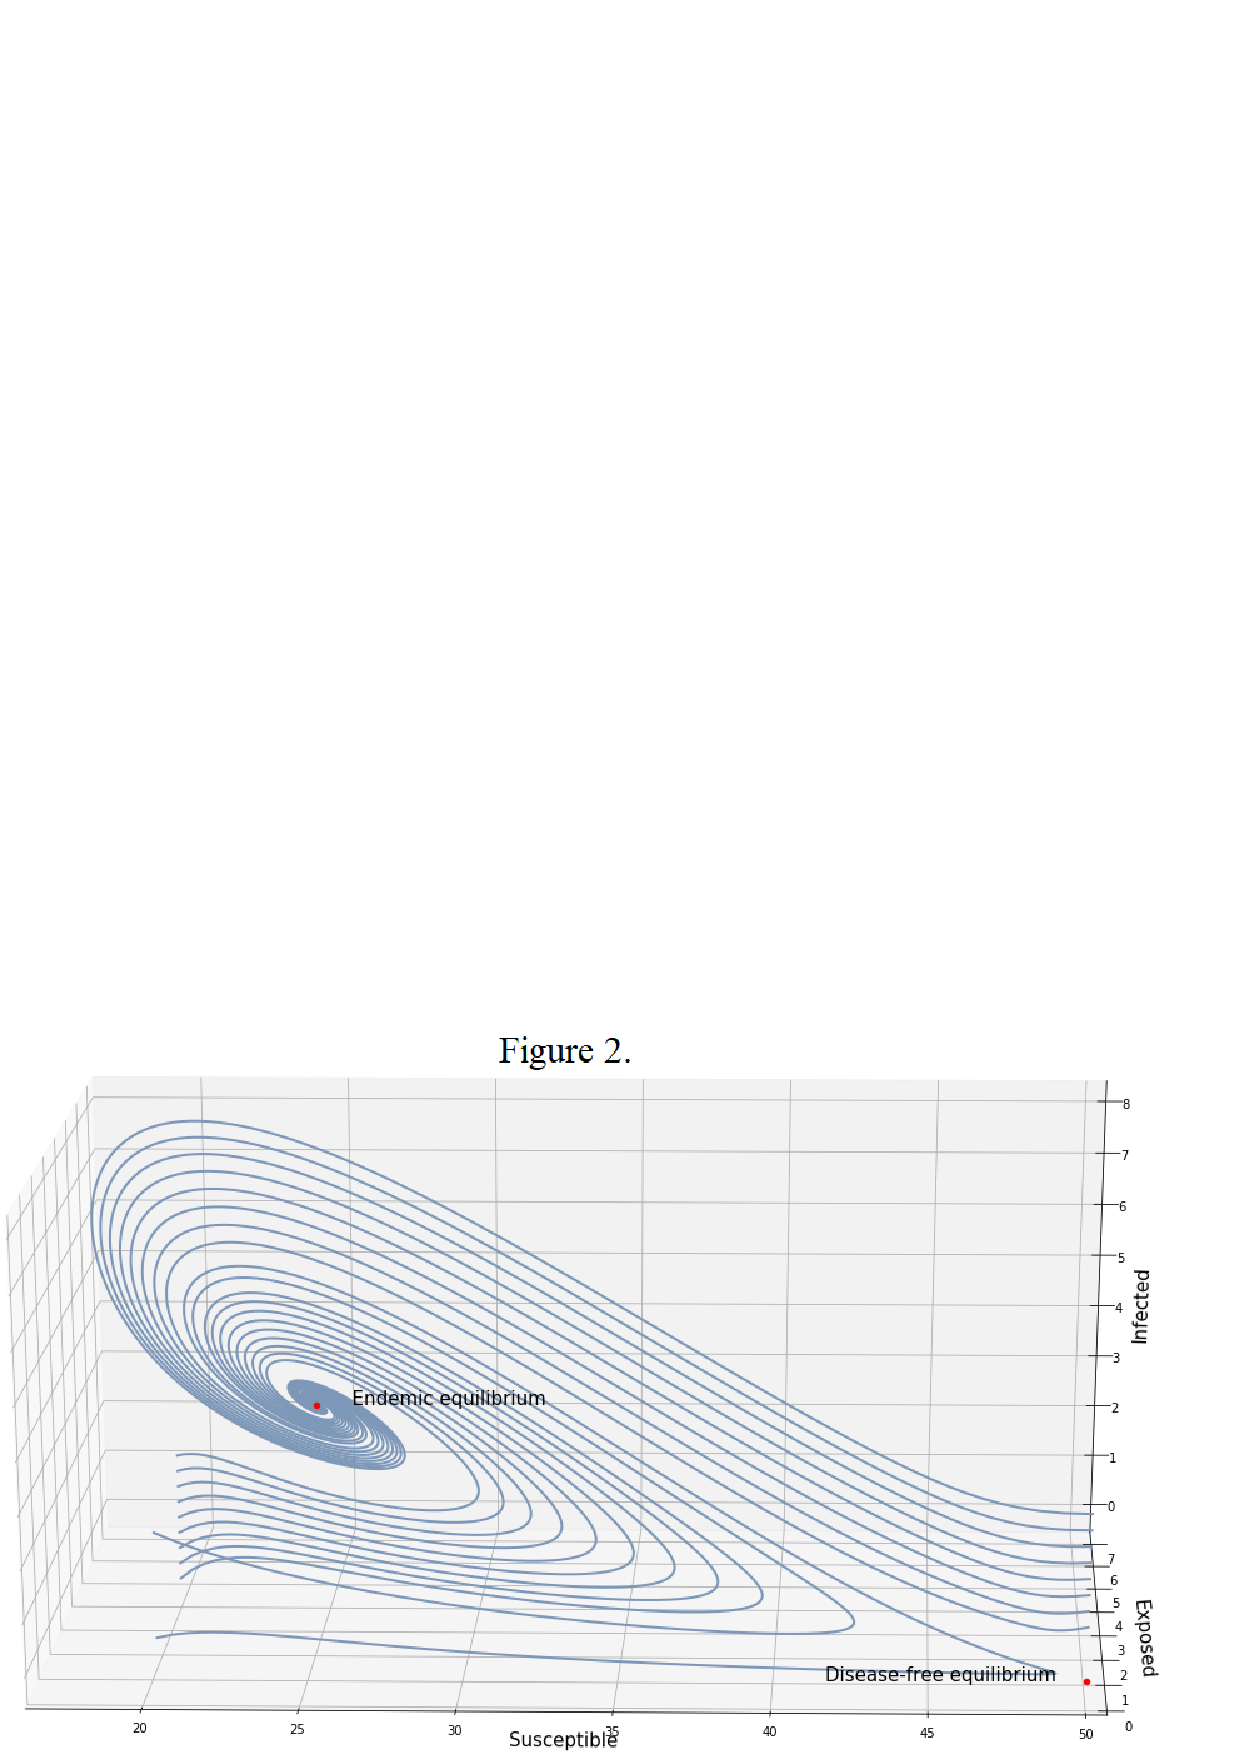
\includegraphics[scale = 0.31]{Endemic_and_Disease_free.png}
\end{tabular}

\begin{tabular}{llll}
\hspace{0.5 em}
&
\includegraphics[scale = 0.3]{Two_Endemic.png}
&
\hspace{3 em}
&
\includegraphics[scale = 0.29]{Bifurcation_b.png}
\end{tabular}
\end{center}
  }
  
\headerbox{Bifurcation Analysis}{name=9,column=1,span=1,below = 6}{
Figure $4$ represents the bifurcation diagram for the parameter $b$. There are two threshold values for $b$ - a Limit Point and a Branch Point, so we can consider the following three cases:\\
\begin{itemize}
    \item When $\mathbf{b < LP}$ we only have one \textbf{\textcolor{imperialblue}{stable disease-free equilibrium}}. In this case the disease \textit{dies out} in time.
    \item When $\mathbf{LP < b < BP}$ we have one \textbf{\textcolor{imperialblue}{stable}} and one \textbf{\textcolor{imperialblue}{unstable endemic equilibria}} and also one \textbf{\textcolor{imperialblue}{stable disease-free equilibrium}}. In this case the disease either \textit{dies our or converges} to an endemic equilibrium (as in Figure 3).
    \item When $\mathbf{b > BP}$ there is one \textbf{\textcolor{imperialblue}{stable endemic equilibrium}} and an \textbf{\textcolor{imperialblue}{unstable disease-free}} one. In this case the disease \textit{doesn't die out} in time.
\end{itemize}}
\headerbox{Conclusion}{name=7,column=2,span=1,below = 6}{
This paper considers an SEIR model with limited hospital treatment. We deduce that there can be either $(1)$ no endemic equilibrium - disease dies out, $(2)$ one stable endemic equilibrium and one unstable disease-free equilibrium or $(3)$ two endemic equilibria - one stable and one unstable. In order for the disease to die out, we can reduce $R_0$ below $R_0^{*}<1.$ This can be done by reducing the $b$ parameter or, in other words, by improving medical conditions.
\vspace{0.37 em}
} 


\headerbox{References}{name=8,column=2,span = 1, below = 7}{
    \printbibliography[heading=none]
  }

\end{poster}

\end{document}
